% !TEX root = ../main.tex
\subsubsection{Alignment Effect}
\label{14.11::alignment_effect}
    % Introduction: The problem.
    The data from the RG-F experiment is divided based on the season in which the runs take place, namely Spring 2020 and Summer 2020.
    According to the run group's guidelines, it is recommended to use Summer data as it has undergone more calibration compared to the Spring data.
    However, the calibration work conducted so far does not include the FMT detector, resulting in a significant misalignment effect.

    % Cause of the problem.
    Through simple visual inspection, two distinct peaks can be clearly observed between $z = -36$ cm and $z = -30$ cm in figure \ref{fig::12.41::dc_vs_fmt_vz_11983}.
    The leftmost peak corresponds to the scattering chamber window, while the second peak corresponds to the RG-F target window.
    These peaks appear merged in figure \ref{fig::14.10::vz_012933}.
    As discussed in section \ref{12::fmt_alignment_and_reconstruction}, this issue arises due to the lack of correction for FMT misalignments.

    % Solution.
    The simplest solution is to utilize Spring data.
    Although more calibration work has been performed on the Summer data, it mainly pertains to the CD, which is not used in this analysis.
    Figure \ref{fig::14.11::vz_012016} depicts the same $v_z$ plot from Spring 2020 run 12016, where both peaks are clearly visible.
    This indicates that the misalignment issue has been appropriately addressed in that particular run.

    \begin{figure}[t!]
        \centering\frame{
        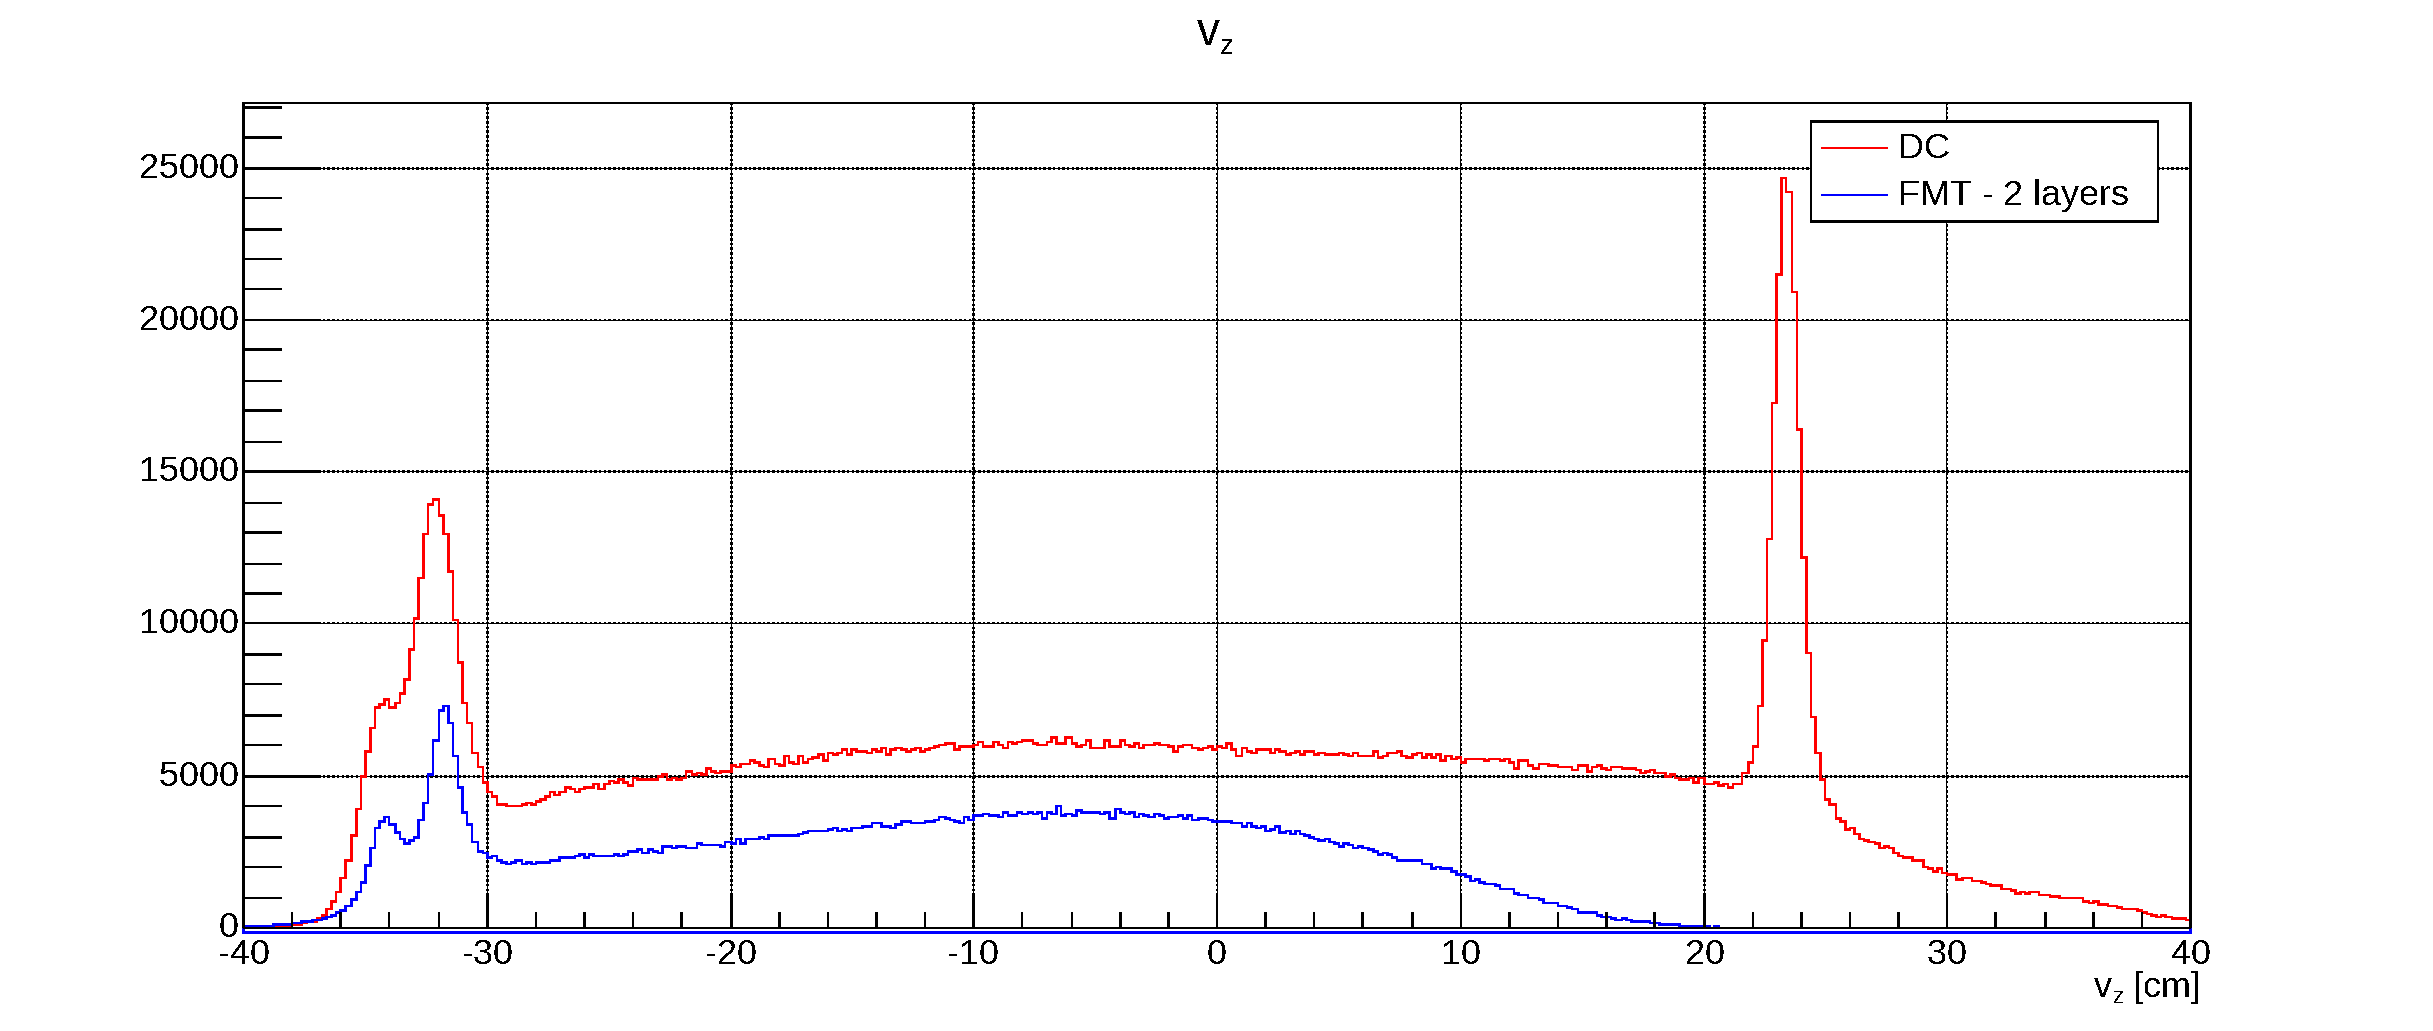
\includegraphics[width=\textwidth]{11vz_012016.pdf}}
        \caption[$v_z$ for DC and FMT, run 12016]{$v_z$ for DC (in red) and FMT (in blue). Spring 2020 data, run 12016. The upstream twin peaks can be clearly distinguished, suggesting a correct misalignment correction.}
        \label{fig::14.11::vz_012016}
    \end{figure}
